\subsection{Modelo de Android}
\begin{frame}
 \begin{center}
  \LARGE Modelo de Android
 \end{center}
\end{frame}
\begin{frame}
 \frametitle{Modelo de Android}
 {Android es un sistema operativo de código abierto, diseñado para dispositivos móviles y desarrollado por Google junto con la Open Handset Alliance.}\pause
 \begin{figure}[H]
    \centering
    \begin{subfigure}{0.75\linewidth}
		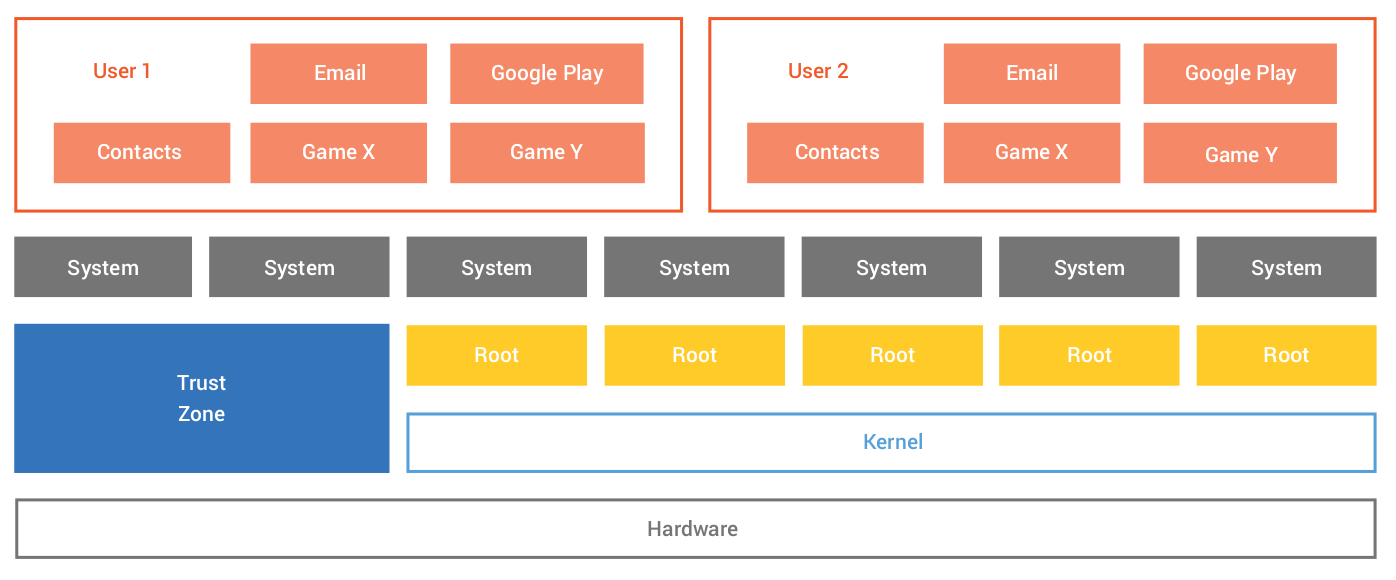
\includegraphics[width=\linewidth]{android_security_model}
	    \label{fig:ch01:sandbox}
    \end{subfigure}
    \caption{Aislamiento de las aplicaciones según su UID.}
 \end{figure}
\end{frame}
\begin{frame}
 \frametitle{Modelo de Android}
 \begin{small}
 \begin{itemize}[<+->]
     \item Podemos clasificar los permisos según el riesgo implícito al otorgarlos:
     \begin{multicols}{2}
     \begin{itemize}[<+->]\small
      \item \emph{\textbf<6->{Normal}}
      \item \emph{\textbf<6->{Dangerous}}
      \item \emph{\invisible<6->{Signature}}
      \item \emph{\invisible<6->{Signature/System}}
     \end{itemize}
     \end{multicols}\pause
     \item A partir de la versión 6.0 se propone un nuevo modelo de permisos:\pause
         \begin{figure}[btp]
            \begin{subfigure}{0.4\linewidth}
            \centering
                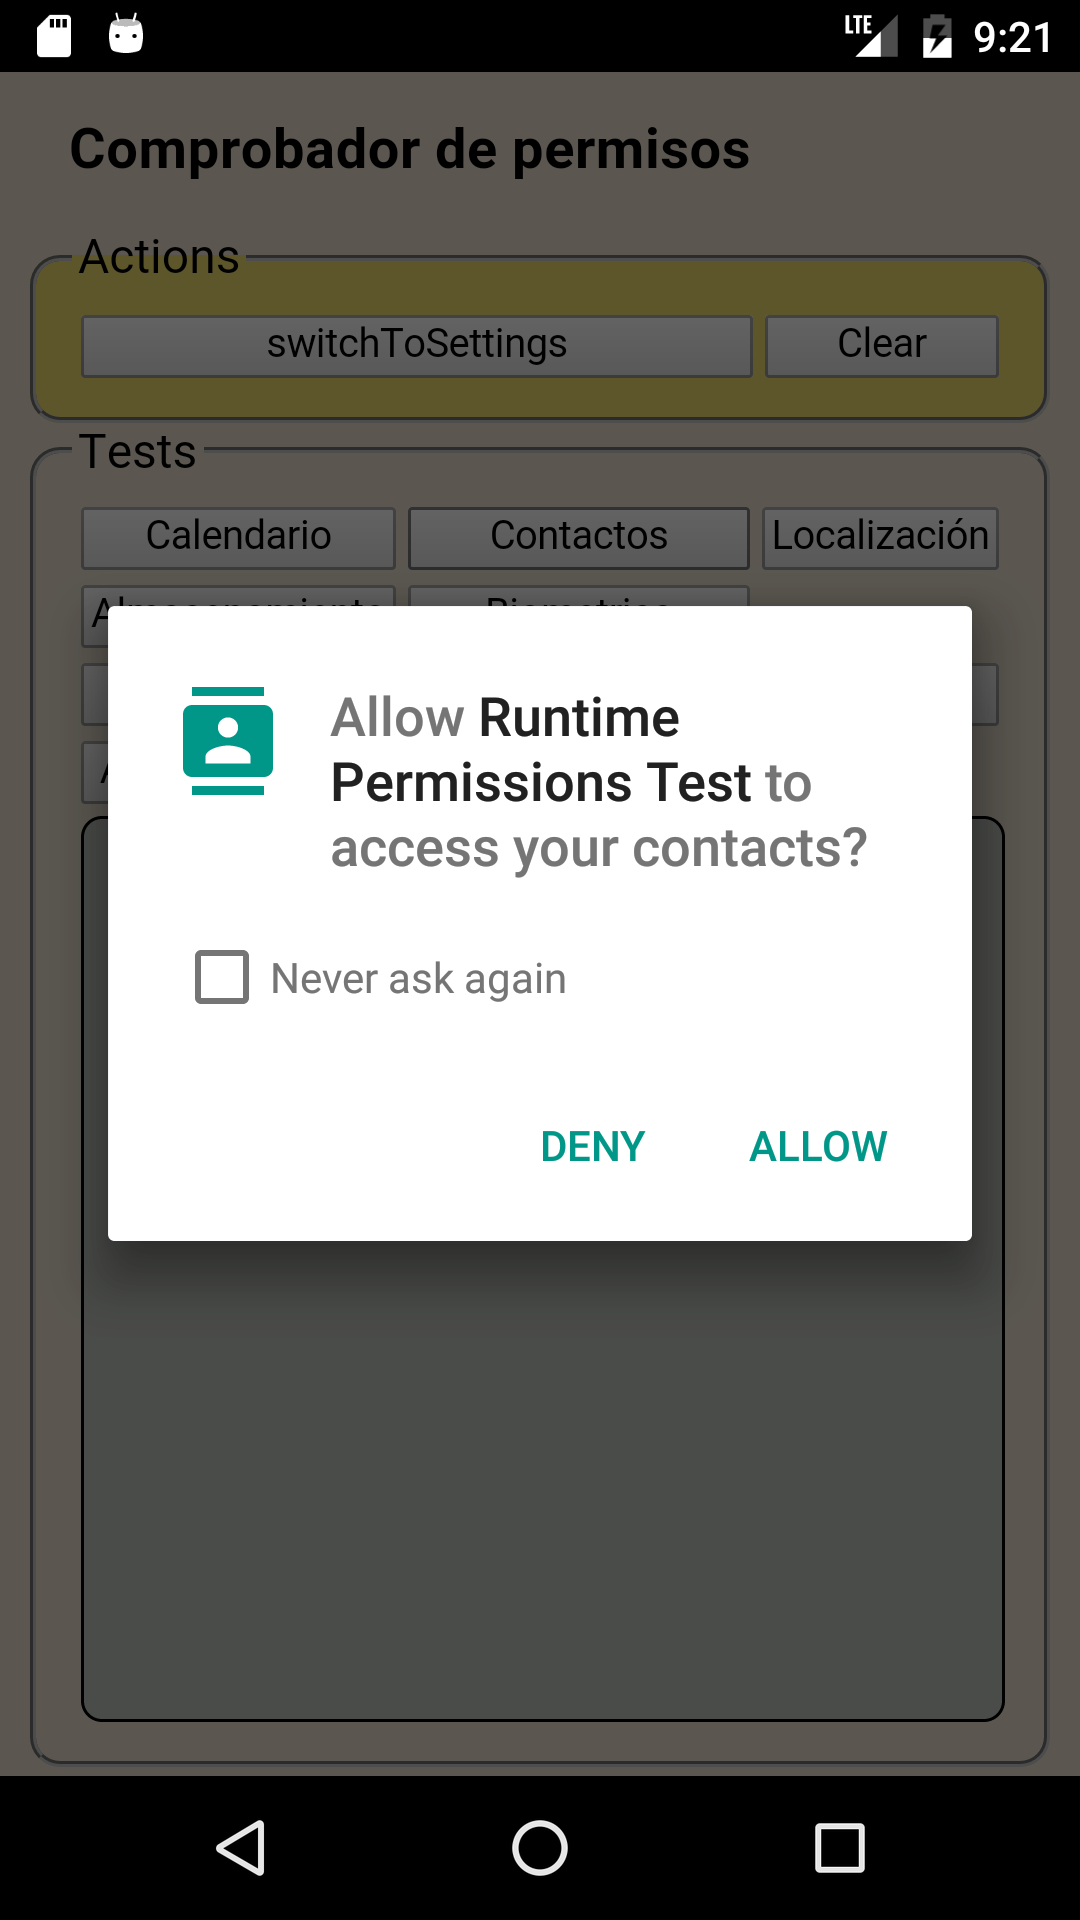
\includegraphics[width=.5\linewidth]{allow_contact}
                \caption{Solicitud de un permiso.}
            \end{subfigure}
        \begin{subfigure}{0.4\linewidth}\pause
        \centering
            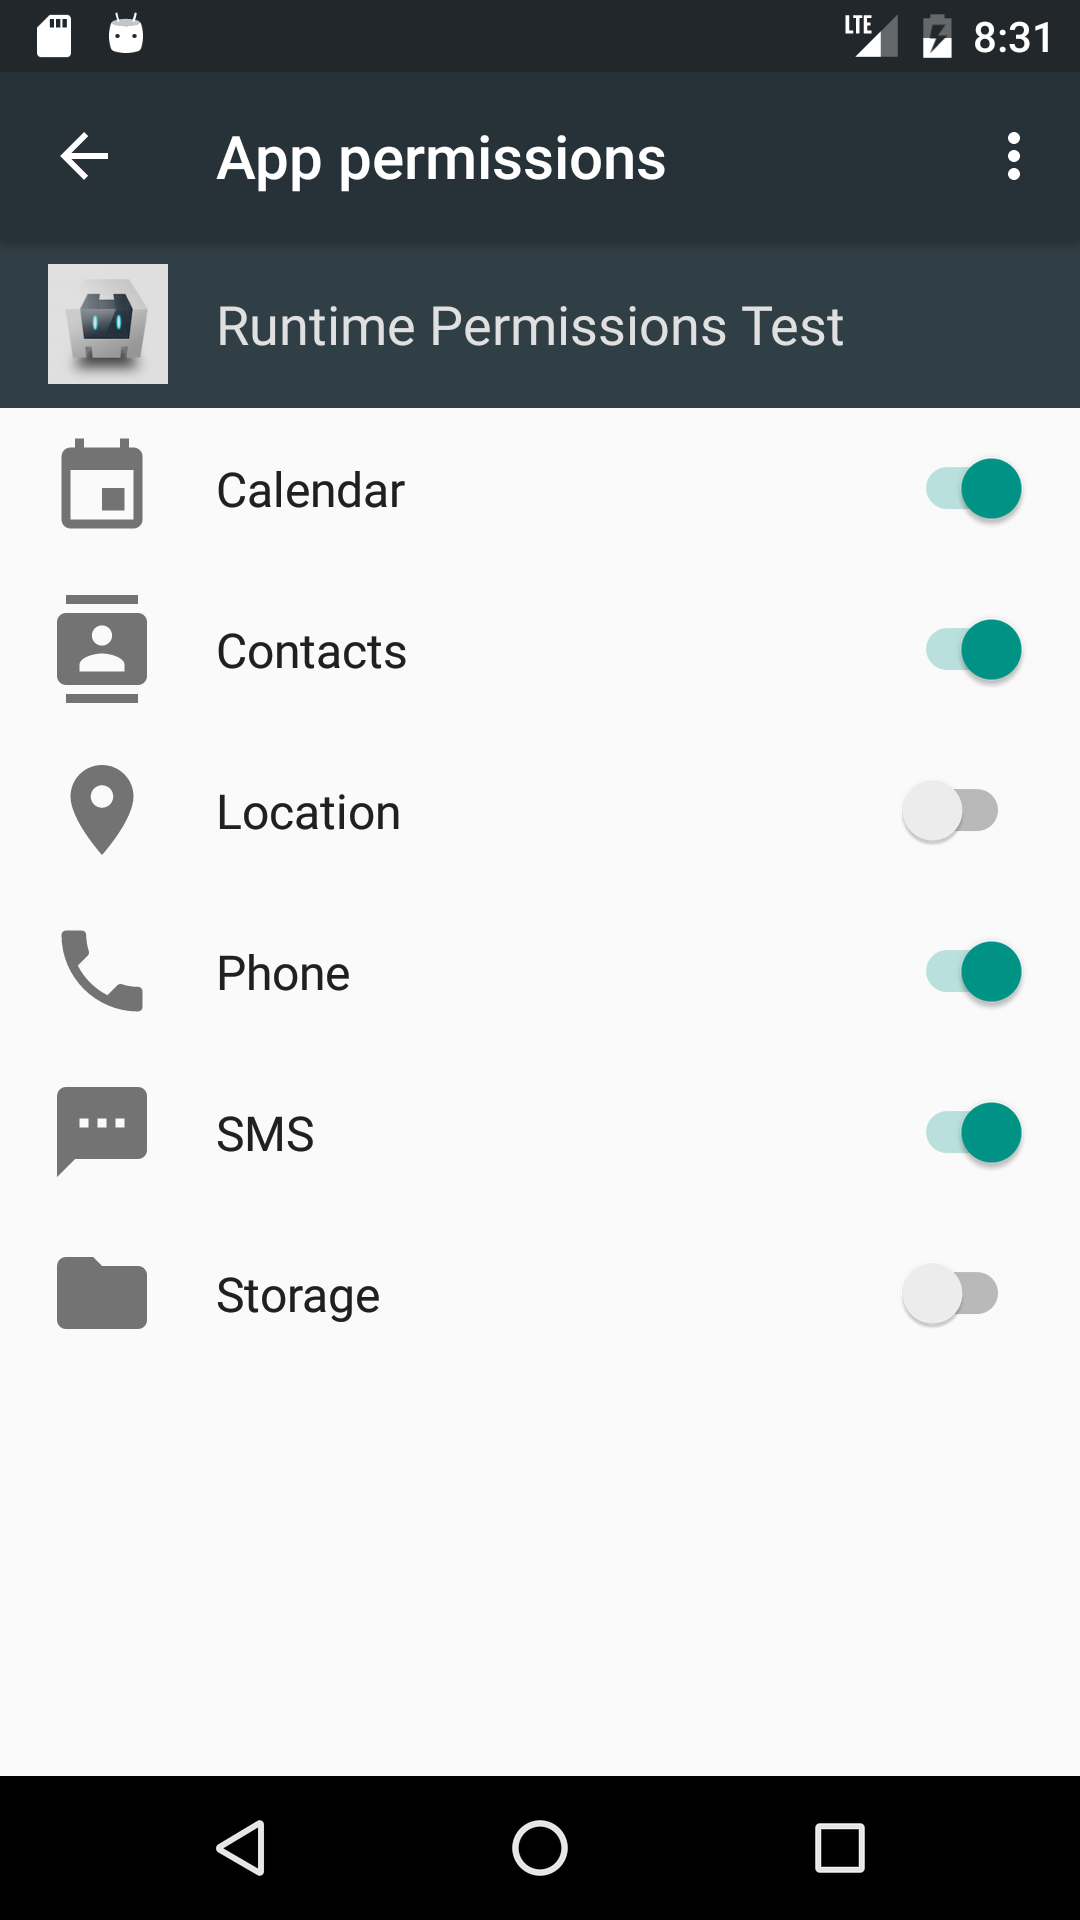
\includegraphics[width=.5\linewidth]{app-permissions}
            \caption{Listado de los permisos.}
    	\end{subfigure}
    	\caption{Nuevo modelo de permisos.}
        \end{figure}
 \end{itemize}
  \end{small}
\end{frame}
